
\documentclass{beamer}
\usetheme{metropolis} % Use metropolis theme





\title{ECON 3818: Introduction to Statistics with Computer Applications}
%\subtitle
\date{\today}
\author{Kyle Butts}



\definecolor{blue}{RGB}{0,114,178}

\definecolor{red}{HTML}{EB0E09}
\definecolor{yellow}{RGB}{240,228,66}
\definecolor{green}{RGB}{0,158,115}
\definecolor{maroon}{HTML}{AF3335}
\definecolor{purple}{HTML}{7E90B8}


\definecolor{mybackground}{HTML}{ECECEC}
\setbeamercolor{background canvas}{bg= mybackground}

\definecolor{buff-gold}{HTML}{CFB87C}
\definecolor{buff-grey}{HTML}{565A5C}
\definecolor{buff-lightgrey}{HTML}{A2A4A3}
\definecolor{buff-black}{HTML}{000000}

\setbeamercolor{alerted text}{fg=buff-gold!80!black}
\setbeamercolor{frametitle}{bg=buff-black}
\setbeamercolor{title}{fg=buff-grey}
\setbeamercolor{button}{bg=buff-gold}

% Allow to remove indent w/ \begin{itemize}[leftmargin= *]
\usepackage{enumitem}
\setlist[itemize]{label= \textbullet}

% \usepackage[libertine]{newtxmath}
\usepackage{longtable}
\usepackage{booktabs}
\usepackage{enumitem}







\begin{document}

% Title Page ---------------------------------------
\maketitle




% Chapter 9 ----------------------------------------
\section{Chapter 9: Producing Data -- Experiments}

\begin{frame}{Observation versus Experiment}
	Experiments don't just observe individuals or ask them questions. They actually impose some treatment in order to measure the response
	\begin{itemize}
		\item An \alert{observational study}: observe individuals and measures variables of interest
		      \begin{itemize} 
		      	\item Does not attempt to influence response 
		      	\item Describe some group or situation
		      	\item Example: Current Population Survey
		      \end{itemize}
		\item An \alert{experiment}: deliberately imposes some treatment on individuals to observe their responses
		      \begin{itemize}
		      	\item Purpose is to study whether treatment causes a change in response 
		      	\item Example: Giving families in developing countries money if they keep their kids in school longer
		      \end{itemize}
	\end{itemize}
\end{frame}

\begin{frame}{Problem with Observational Studies}
	The main issue with simply observing people is the issue of \alert{confounding variables}
	
	\begin{itemize}
		\item \alert{explanatory variable}: a variable included and accounted for in the experiment/analysis 
		\item \alert{lurking variable}: also known as an omitted variable; it is not included in the sample yet it influence response variable that are in the sample 
	\end{itemize}
\end{frame}

\begin{frame}{Confounding Variables}
	Example: A study is trying to determine whether playing violent video games increases aggressive/violent behavior.
	\begin{center}
		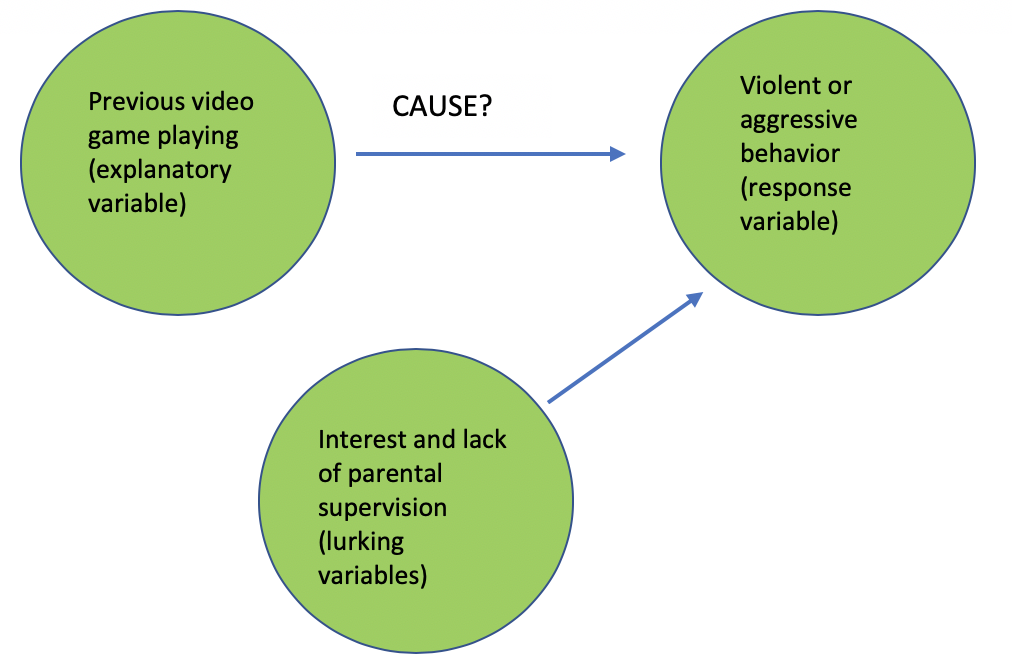
\includegraphics[width=0.8\textwidth]{lurking_example}
	\end{center}
\end{frame}

\begin{frame}{Confounding Variables}
	In that study,  you are comparing people who chose to play video games and those that do not. The effect of playing video games is confounding with the characteristics who choose to play more video games.
	
	These differences between the type of people who choose to play or not play video games, makes determining the \textit{true} effects of playing video games hard to tease out
\end{frame}


\begin{frame}{Dealing with Confounding Variable}
	Experiments seek to resolve the issue of confounding variables. Observational studies often suffer from confounding effects because they don't (or can't) measure lurking variables
	\begin{itemize}
		\item Well-designed experiments avoid confounding effects by measuring lurking variables directly or creating an environment where they are no longer relevant
	\end{itemize}
\end{frame}

%\begin{frame}{Visualizing Confounding Issue}
%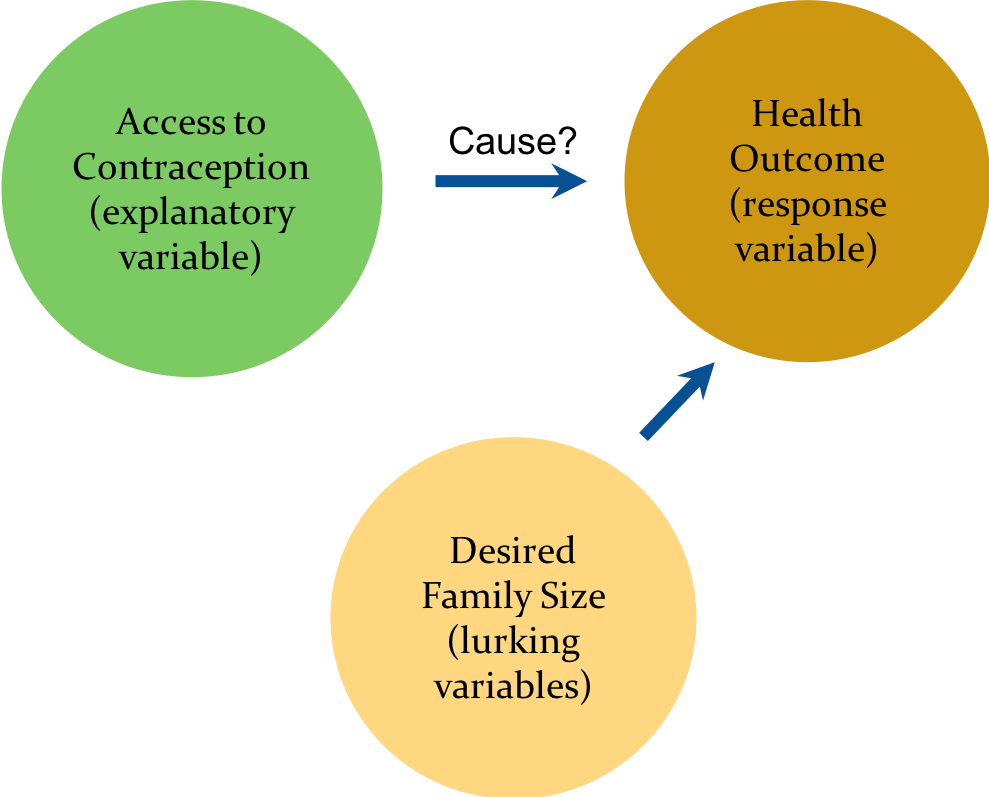
\includegraphics[width=0.8\textwidth]{confounding}
%\end{frame}

\begin{frame}{Experiment Terminology}
	An \alert{experiment} is a statistical study in which we actually implement a \alert{treatment} to \alert{subjects} to observe their \alert{response}
	\begin{itemize}
		\item A \textit{treatment} is any specific experimental condition applied to the subjects
		\item \textit{subjects} refers to the individuals (people, animal, objects) being studied
		\item The explanatory variables in an experiment are often called \textit{factors}
	\end{itemize}
\end{frame}

\begin{frame}{Poorly Designed Experiments}
	
	Experiments don't guarantee good data -- good designs are essential
	\begin{itemize}
		\item Example: A college regularly offers a course to prepare students for the GMAT. This year it will only offer an online version of the course.
		      
		\item If the results are 10\% higher this year than last year. Can we conclude the online course is more effective?
	\end{itemize}
	
\end{frame}

\begin{frame}{Poorly Designed Experiments}
	
	Experiments that don't have \alert{randomized treatments} are highly susceptible to confounding effects
	\begin{itemize}
		\item Separating sample into \textit{treatment} and \textit{control} groups helps with this issue. Comparison of the outcomes across the two groups is less likely to be confounding
		      
		\item this is called a \alert{randomized comparative experiment}
	\end{itemize}
	
\end{frame}

\begin{frame}{Randomized Comparative Experiments}
	
	Proper \alert{randomization} leads to treatment and control groups that are similar before any treatment is applied. 
	
	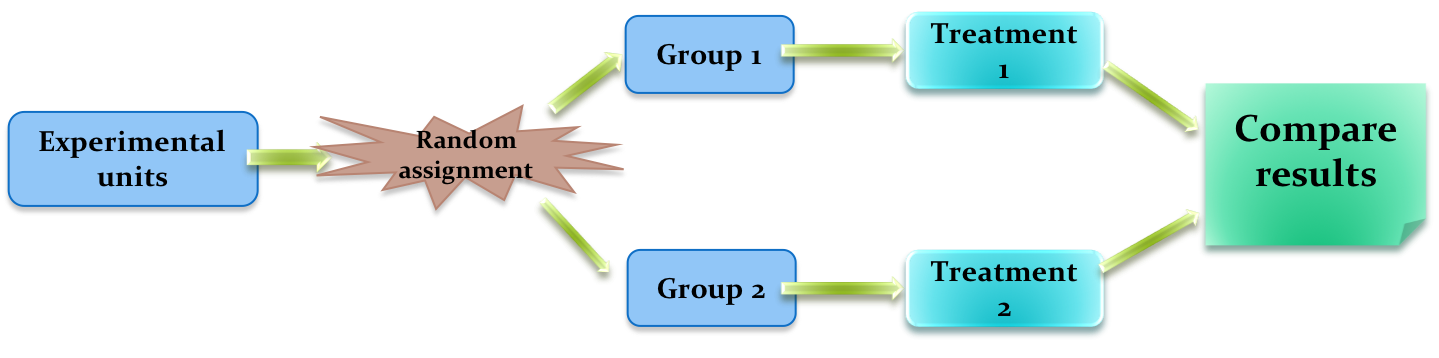
\includegraphics[width=\textwidth]{randomassignment}
	
	If assignment is truly random, then the difference in average response must be due to either the treatment 
	
\end{frame}

\begin{frame}{Randomized Comparative Experiment}
	Correct way to test difference between classroom versus online GMAT course. Given 50 students need to take the course, list them from 1-50 and randomly assign numbers to the two groups -- one that takes the course online and one that takes the course in the classroom. 
	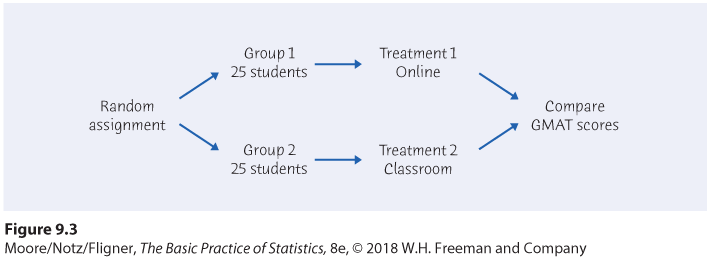
\includegraphics[width=\textwidth]{randomized_GMAT}
\end{frame}


\begin{frame}{Ways to Properly Randomize}
	The log of a randomized comparative experiment depends on our ability to treat all the subjects the same in every way, except for the actual treatments being compared
	\begin{itemize}
		\item \alert{Placebo}: gives the real treatment to one group, and a fake (but similar) treatment to the other group
		\item \alert{Double-Blind}: neither the subjects nor the experimenters know which treatment each subject is receiving 
		\item \alert{Matched-Pairs}: compares two treatments, where the subjects are as closely matched as possible. 
		\item \alert{Block design}: a block is a group of individuals that are known to be similar in some way. A block design randomly assigns individuals separately within each block. 
	\end{itemize}
\end{frame}



\begin{frame}{Experiments in Economics}
	\textbf{2019 Nobel Prize in Economics: Abahjuit Banerjee and Esther Duflo}
	
	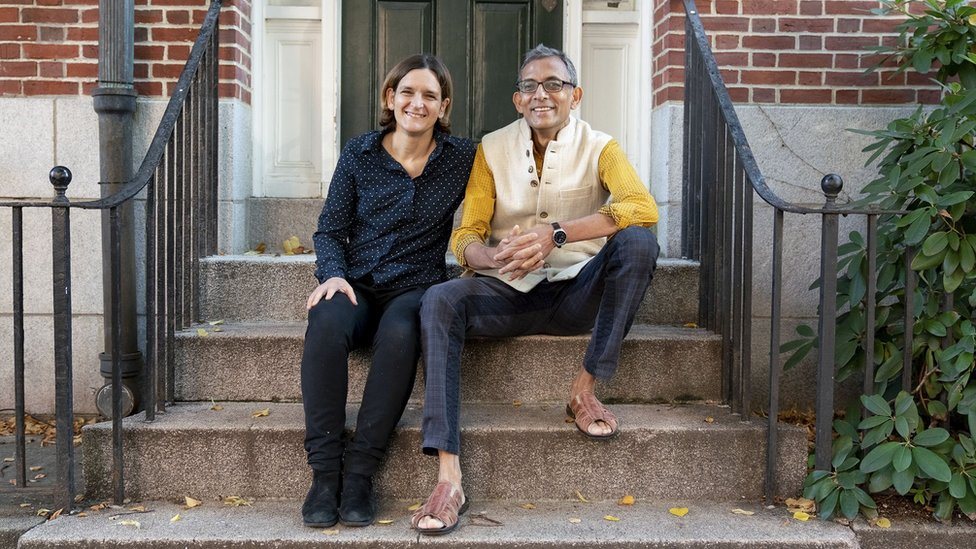
\includegraphics[width = \linewidth]{duflo_and_banerjee.jpg}
\end{frame}

\begin{frame}{Duflo and Banerjee}
	\begin{itemize}
		\item Duflo and Banerjee focus on developing countries and run many small-scale experiments 
		
		\item Does Microfinancing work? They find it \textit{really} depends on the loan structure.

		\item How to improve education outcomes? Computers and supporting family income are highly effective. 

		\item Improving government services. Large-scale experiments to test how to best distribute funding. 
		
		\item https://www.nobelprize.org/prizes/economic-sciences/2019/duflo/lecture/
	\end{itemize}
\end{frame}

\begin{frame}{Matched Pairs Example}
	How much does schooling improve wages?

	\begin{itemize}
		\item Confounding Variables: family characteristics, like income, intelligence, and parental education levels.
	\end{itemize}
	
	Krueger and Ashenfelter went to an Ohio Twins Festival to survey twins. By comparing twins, you can avoid many omitted (lurking) variables regarding family characteristics.

	They are able to better quantify the increase in wages due to schooling directly. 

	\textit{Krueger and Ashenfelter, 1994. ``Estimates of the Economic Return to Schooling from a New Sample of Twins,'' American Economic Review}
\end{frame}


\begin{frame}{Natural Experiments: Family Wealth}	
	Does family wealth improve childhood outcomes?
	
	\begin{itemize}
		\item Possible confounding variables: parents profession, education levels, and economic connections.
	\end{itemize}
	
	Bleakley and Ferrie (2016) look at Georgia’s Cherokee Land Lottery of 1832 which was a lottery that gave away large plots of land. 
	
	They find that family wealth has no effect on childhood education outcomes, i.e. confounding variables explain why wealthier families have improved childhood outcomes

	\textit{Bleakley and Ferrie, 2016. ``Shocking Behavior: Random Wealth in Antebellum Georgia and Human Capital Across Generations,'' Quarterly Journal of Economics}
\end{frame}

\begin{frame}{Natural Experiments: Fetal Health}
	How does poor fetal health affect long-run outcomes?

	\begin{itemize}
		\item Confounding variables: family income!
	\end{itemize}	

	This is a question that can't be answered with a true experiment (can not randomly assign this treatment).

	Almond (2006) compares babies born just before and just after the Influenze of 1918. Those born during the Influenze display ``reduced educational attainment, increased rates of physical disability, lower income, lower socioeconomic status''

	\textit{Douglas, 2006. ``Is the 1918 Influenza Pandemic Over?,'' Journal of Political Economy}
\end{frame}

\begin{frame}{Natural Experiments: Medicaid}
	Did Medicaid reduce childhood mortality?

	\begin{itemize}
		\item Confounding Variables: family income, local pollution, disabilities that would lead to being on Medicaid
	\end{itemize}

	Goodman-Bacon uses variation in Medicaid rollout to compare children who are eligible for Medicaid. He finds that Medicaid indeed reduced childhood mortality with a particularly strong effect among non-white children (a decrease of 11\%).

	\textit{Goodman-Bacon, 2018. ``Public Insurance and Mortality: Evidence from Medicaid Implementation,'' Journal of Political Economy}
	

\end{frame}


\begin{frame}{Block Design Example}
	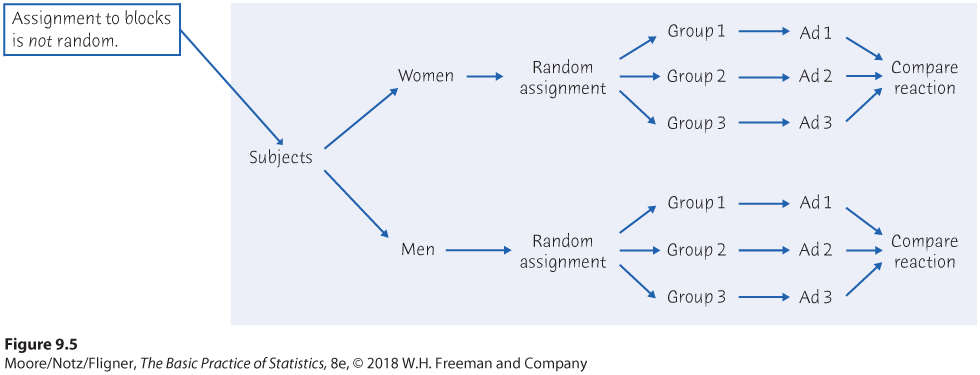
\includegraphics[width=\textwidth]{block_design}
	Since men and women respond differently to advertisement, the company may want to conduct experiment on men and women separately.
\end{frame}

\begin{frame}{Clicker Question}
	\small{An educator wishes to study the effects of sleep deprivation on the ability to concentrate. He decides to study the students in a calculus class. After consultation with a statistician, the educator decides to randomly allocate students to either a group that will sleep for 8 hours the night before class or 6 hours. The educator does not know which group a student belongs to when she or he comes to class. The educator, after talking to some students and before the experiment, decides that the number of classes students have on the same day before calculus could potentially confound the study and wishes to make an adjustment. The design that allows for such an adjustment is called:
		\begin{enumerate}[label=(\alph*)]
			\item randomized block design
			\item placebo controlled randomized design
			\item double-blinded design
			\item matched block design
		\end{enumerate}}
\end{frame}

\begin{frame}{Clicker Question}
	\small{An insurance company wonders whether sports cars "cause" people to drive too fast, or whether those with a propensity for speeding are drawn to sports cars. Researcher has a sample of 100 and randomly assigns 25 drivers to each of four groups: 1) sports car - white, 2) sports car - red, 3) sedan - white, and 4) sedan - red. The primary research questions are: Do sports cars make people drive faster? Does color make a difference? The result shows that people driving red cars drive faster than those driving white cars. There is no statistically significant difference by type. This conclusion is:
		
		\begin{enumerate}[label=(\alph*)]
			\item wrong, because the stated purpose was to only study type
			\item valid, because this was a randomized study and drivers were randomized on color and type
			\item wrong, because you cannot study two different things, like type and color, at once
			\item valid, because sports cars obviously make people drive fast
		\end{enumerate}}
\end{frame}




\end{document}